\section{Import Input data}
Taking advantage of \scipion software framework, we are going to import the above indicated input data using protocols \scommand{import volumes} and  \scommand{import sequence}. Details about the parameters of these two protocols are shown in tutorial Appendices \ref{app:importVolume} and \ref{app:importSequence}, respectively. 

\begin{itemize}
 \item Volume:\\First open the \scommand{import volumes} protocol (\ffigure{fig:import_volume} (1)), fill in the form and execute it (2), and finally you may visualize the volume (3). By default $Chimera$ \citep{pettersen2004} is used for visualization (\ffigure{fig:chimera_visualization_volume}). It shows the 3D map and the $x$ (red), $y$ (yellow) and $z$ (blue) axes.  
 %  The C2 symmetry is shown, as well as the 45º turn of volume regarding the z axis (blue line).
 
 \begin{figure}[H]
  \centering 
  \captionsetup{width=.7\linewidth} 
  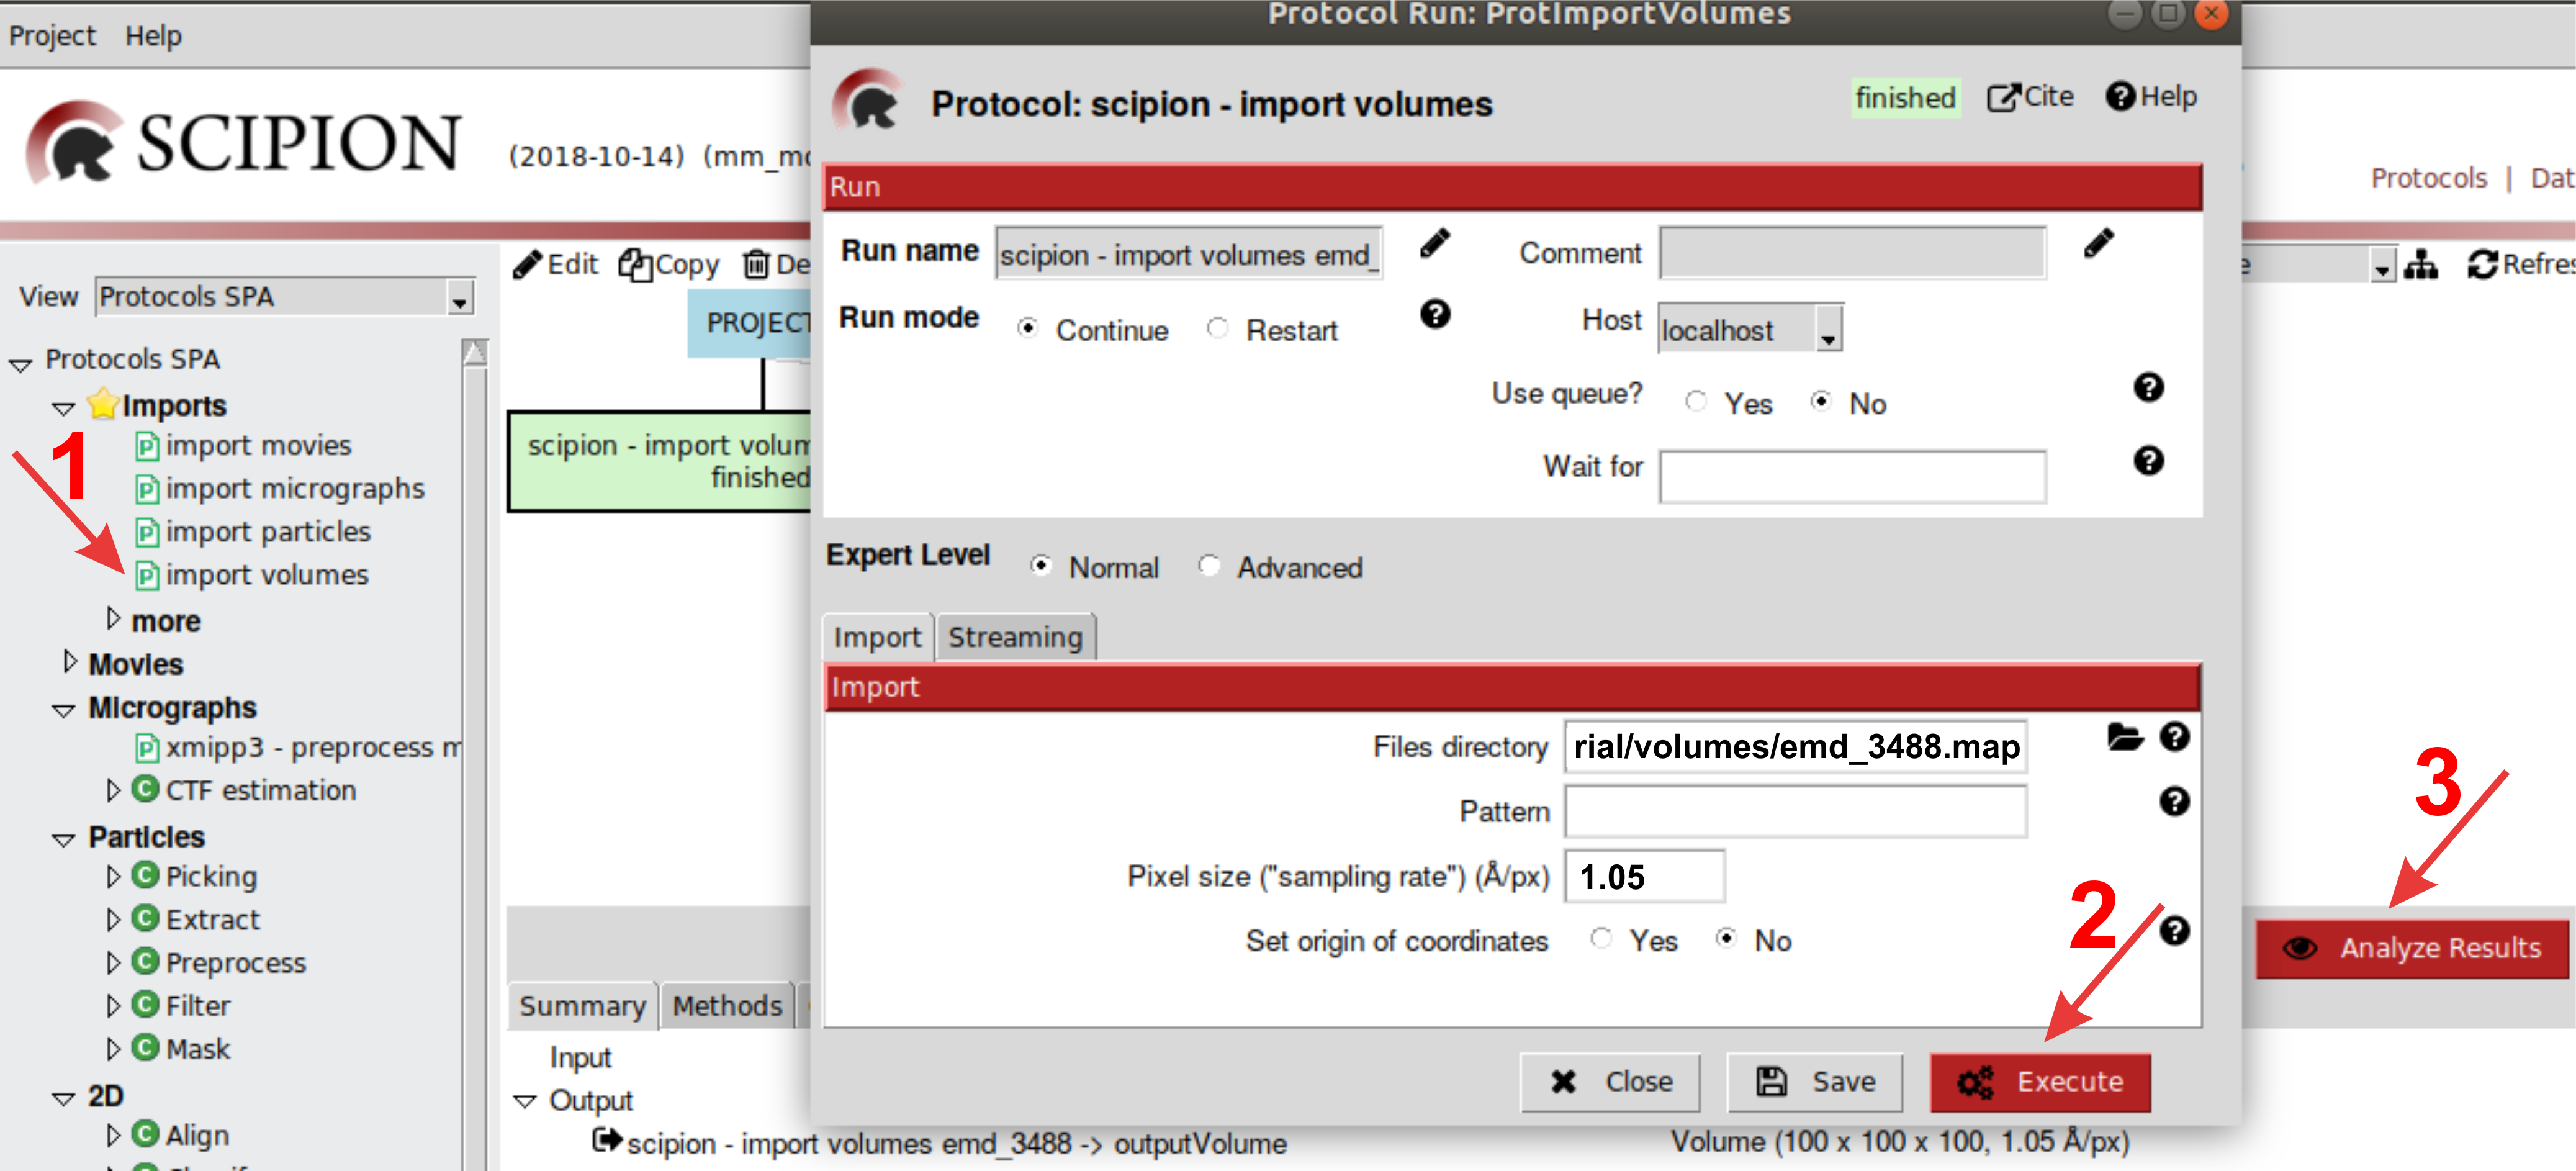
\includegraphics[width=0.80\textwidth]
  {Images/Fig4.png}
  \caption{Importing the volume in \scipion.}
  \label{fig:import_volume}
  \end{figure}
  
 \begin{figure}[H]
  \centering 
  \captionsetup{width=.7\linewidth} 
  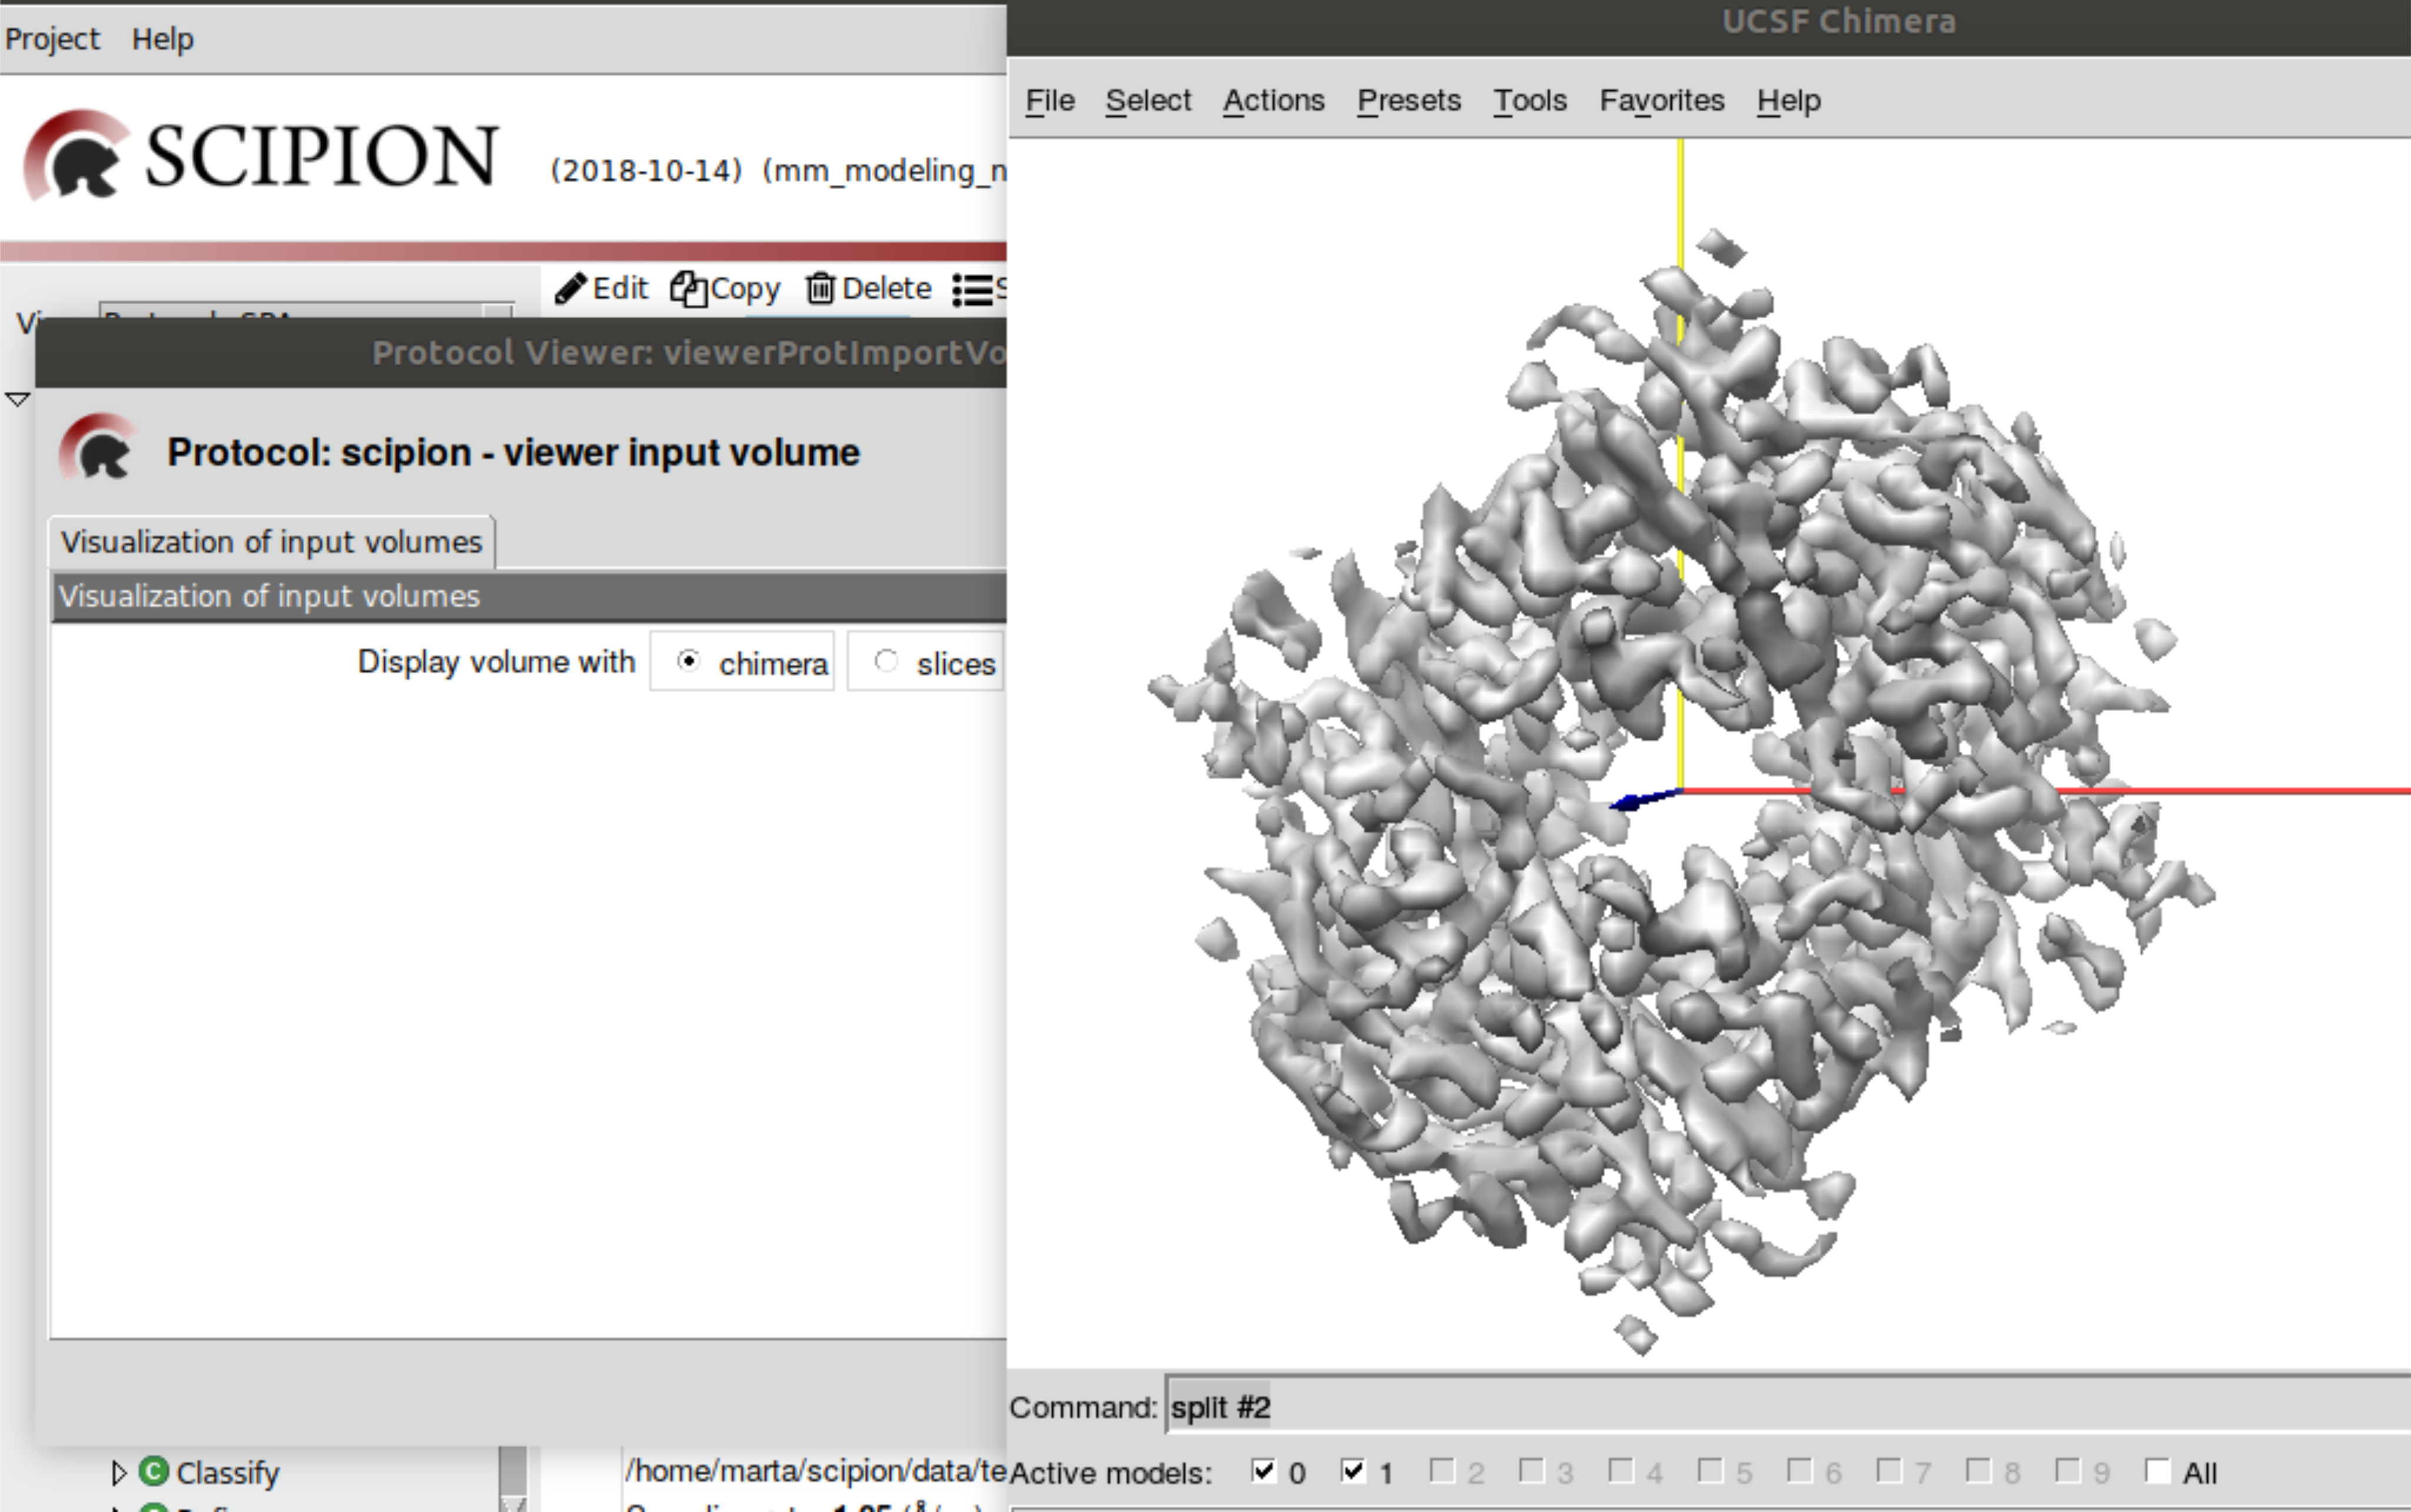
\includegraphics[width=0.80\textwidth]
  {Images/Fig5.png}
  \caption{Volume visualized with $Chimera$.}
  \label{fig:chimera_visualization_volume}
  \end{figure}
 
 \item Sequences:\\
 The sequences of \ttt{Hgb} $\alpha$ and $\beta$ subunits will be independently downloaded from \ttt{UniprotKB}. First of all, open the form of \scommand{import sequence} protocol (\ffigure{fig:import_sequence} (1)), then complete the form to download \ttt{HBA\_HUMAN} protein with \ttt{UniProtKB} accession code \ttt{P69905}, execute the process (2), and finally visualize the sequence (3) in a text editor. The sequence will appear in fasta format as it has been written above. Follow the same protocol to download \ttt{HBB\_HUMAN}.
 
 \begin{figure}[H]
  \centering 
  \captionsetup{width=.7\linewidth} 
  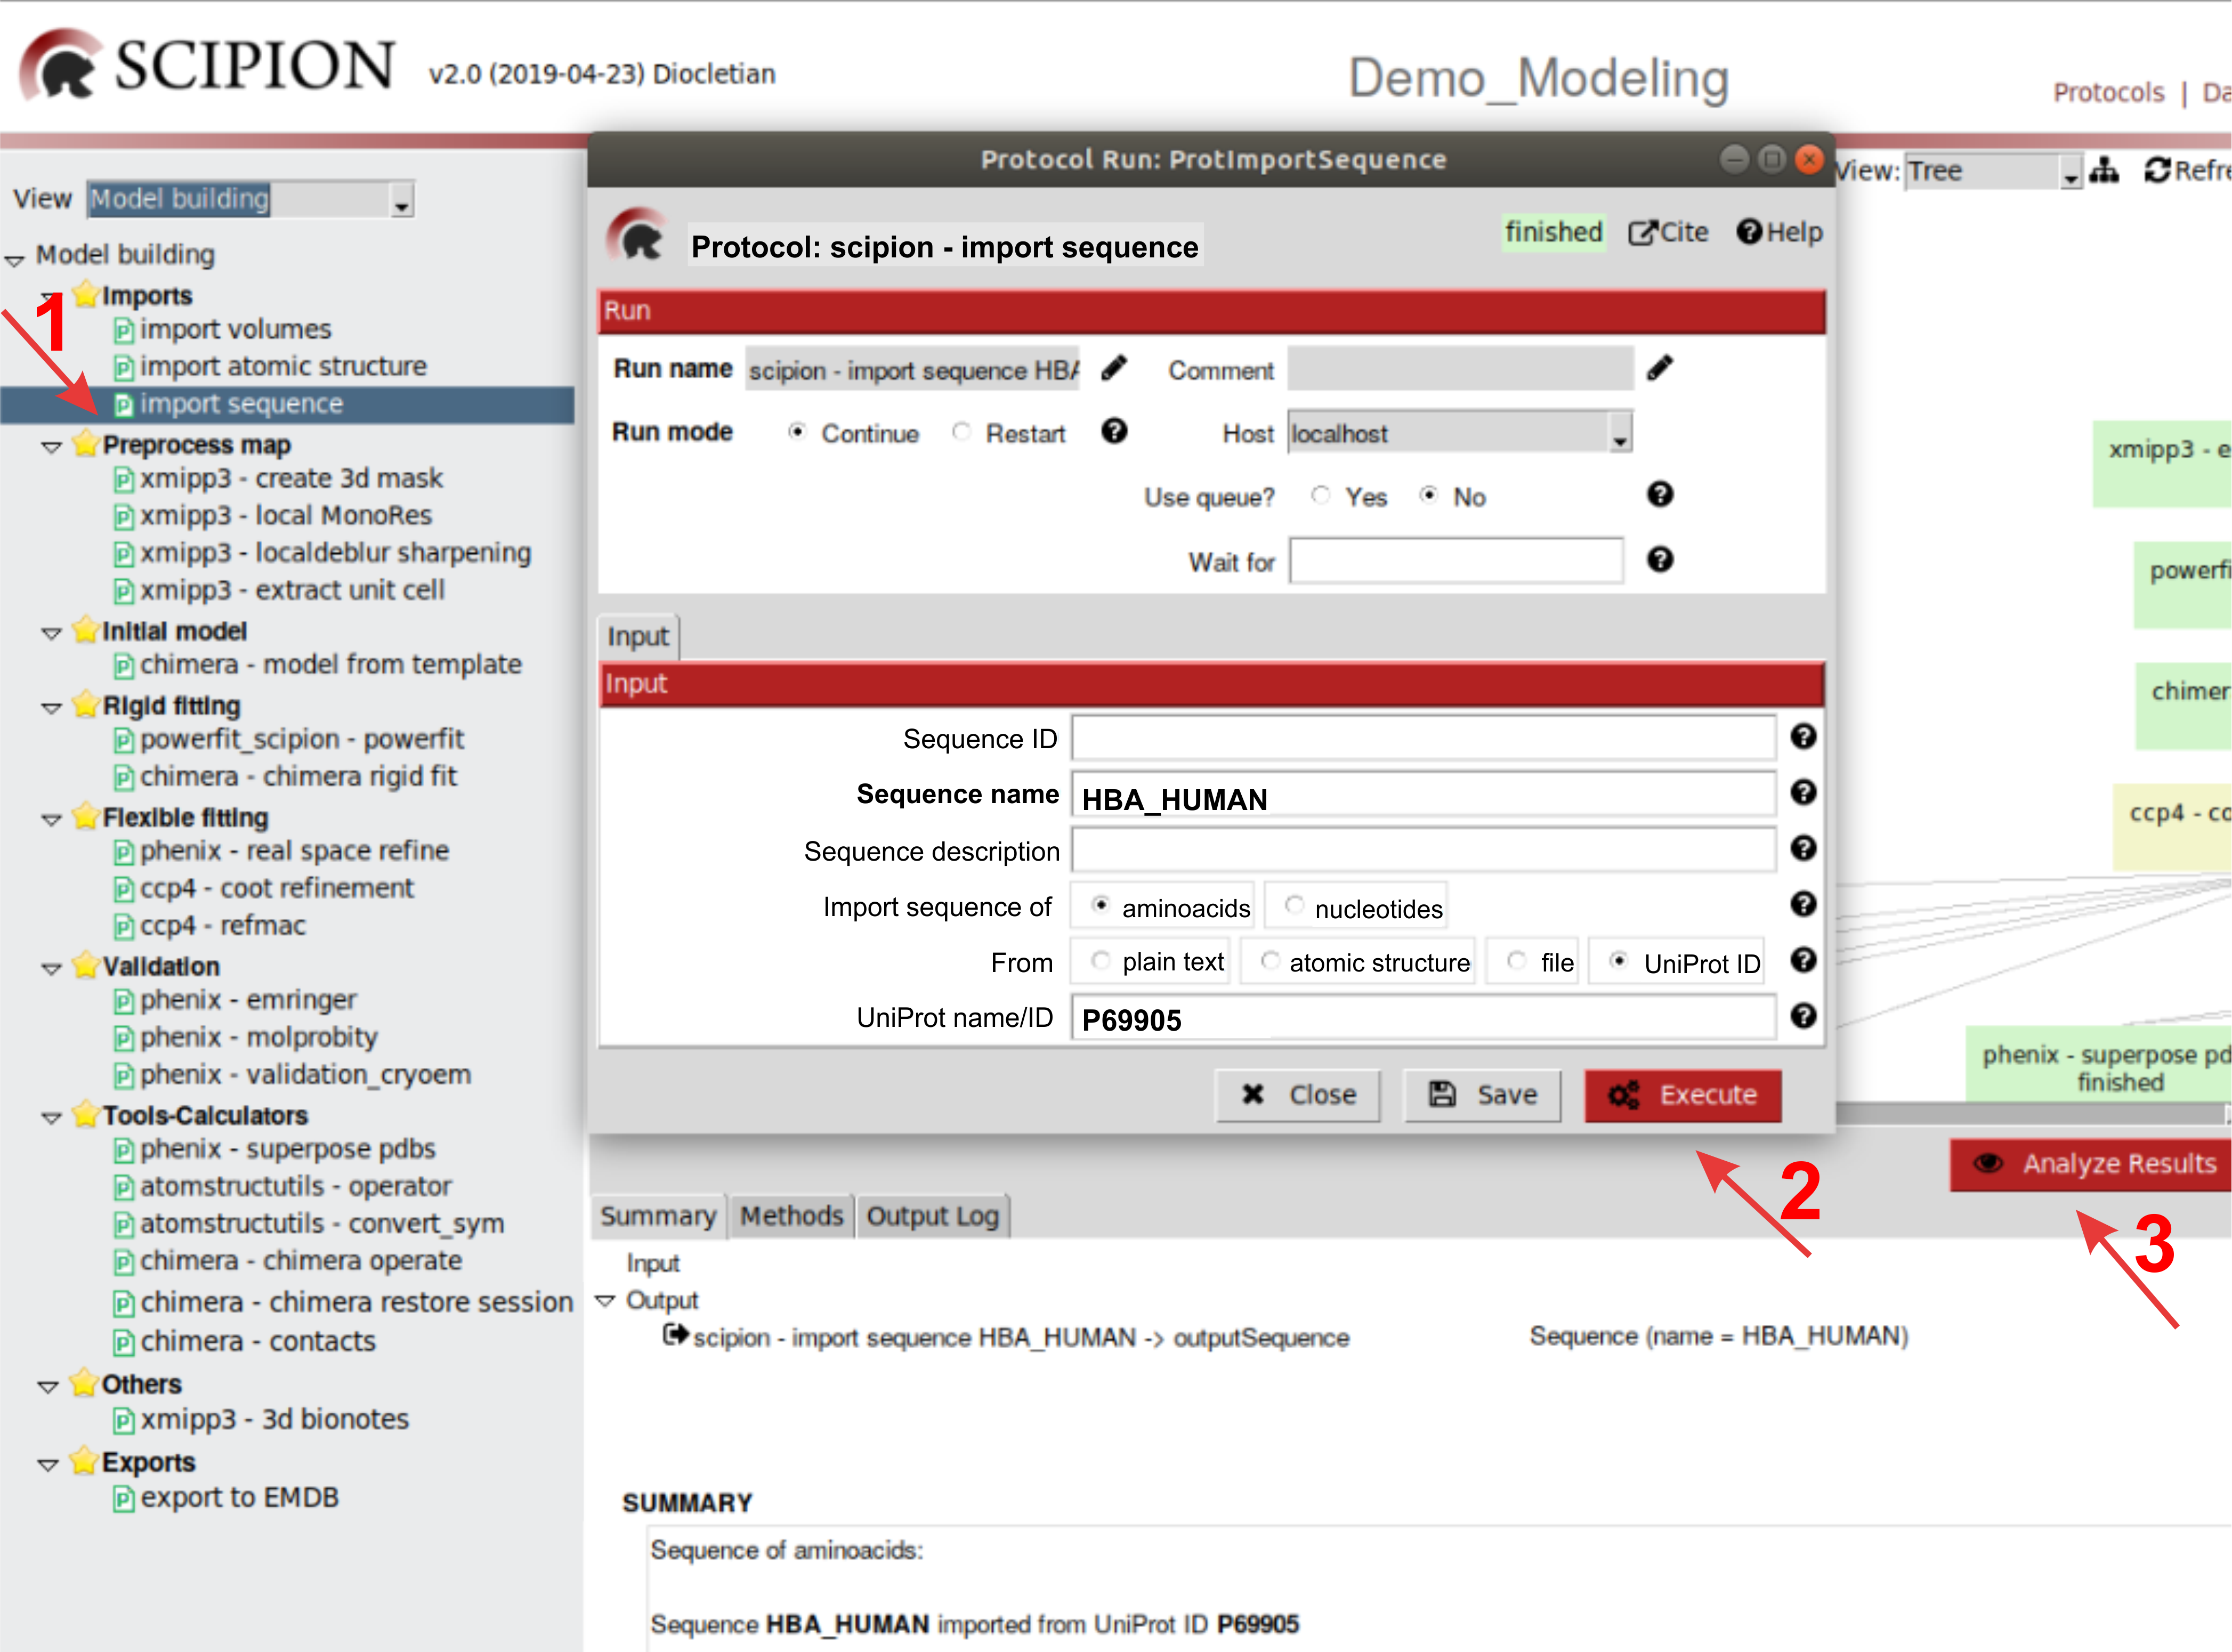
\includegraphics[width=0.80\textwidth]
  {Images/Fig6.png}
  \caption{Importing a \ttt{UniProtKB} sequence in \scipion.}
  \label{fig:import_sequence}
  \end{figure}
 
 \end{itemize}  
